
\begin{wrapfigure}{r}{3.5cm}
\centering
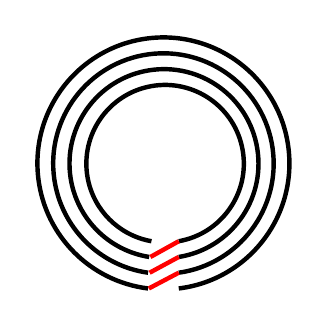
\begin{tikzpicture}[scale = 1]

\draw [ultra thick] (0,0) arc (-80:260:1);
\draw [ultra thick] (0,-0.2) arc (-81:261:1.2);
\draw [ultra thick] (0,-0.4) arc (-82:262:1.4);
\draw [ultra thick] (0,-0.6) arc (-83:263:1.6);

\draw [ultra thick, red] (0,0) -- (-0.36,-0.2);
\draw [ultra thick, red] (0,-0.2) -- (-0.37,-0.4);
\draw [ultra thick, red] (0,-0.4) -- (-0.38,-0.6);

\end{tikzpicture}
\caption{Domain representation with multiple windings.}
\label{fig:winding_geom_scheme}
\end{wrapfigure} 

The algorithm mapping multi-strand and multi-dimensional magnet geometries is explained in this section. Superconducting accelerator magnets are made of a strand or a bunch of strands, e.g. Rutherford cable\footnote{Rutherford cable is a type of an electrical cable used in superconducting technologies reducing Eddy current effects during the ramp up.}, wound multiple times in a certain pattern. Creating a CAD geometry where a single strand domain is wound $n$ times would be a complicated task. Therefore, every winding of the strand is considered as a separate domain, as shown in Fig. \ref{fig:winding_geom_scheme}. The tips of the windings marked in red are coupled with the neighbouring ones thermally and electrically, i.e. they are characterised by the same temperature and voltage. With such an approach, one can easily create multi-strand magnet geometries. Moreover, by specifying which windings are couple together, with the same numerical domain, one can also analyse magnets wound in various manners depending on thermoelectric coupling pattern applied to the winding tips. 

Since the magnet geometry is created, as presented in Fig. \ref{fig:winding_geom_scheme}, one can assume no smooth transition of magnetic field in each winding but rather fixed step values (which may vary in time, though). Since a different value of magnetic field is assigned to each winding, each of them can be characterised by different thermal and electrical material properties. As shown in Fig. \ref{fig:ansys_python_mapping scheme}, the multi-strand geometry is, then, translated into a realistic one-dimensional cable with a length equal to the length of all the windings of a magnet. Each part of this coil length, $L_\text{coil, 1D}$ representing one winding is characterised by a different value of magnetic field field~$B_\text{n}$.

\begin{figure}[H]
\centering
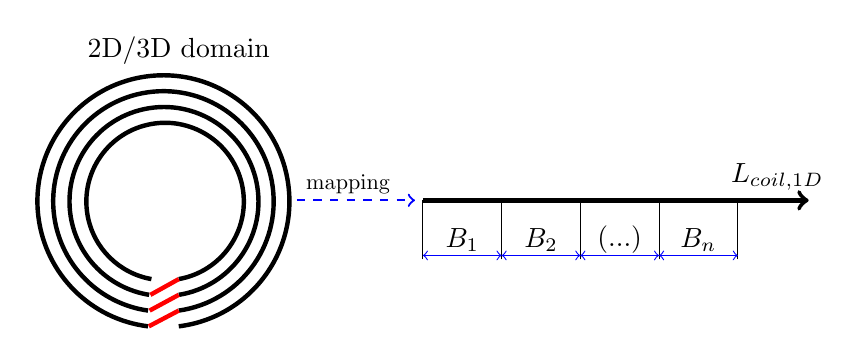
\begin{tikzpicture}[scale = 1]
\draw [ultra thick] (0,0) arc (-80:260:1);
\draw [ultra thick] (0,-0.2) arc (-81:261:1.2);
\draw [ultra thick] (0,-0.4) arc (-82:262:1.4);
\draw [ultra thick] (0,-0.6) arc (-83:263:1.6);
\draw [ultra thick, red] (0,0) -- (-0.36,-0.2);
\draw [ultra thick, red] (0,-0.2) -- (-0.37,-0.4);
\draw [ultra thick, red] (0,-0.4) -- (-0.38,-0.6);
\node[scale = 1.0] at (0,2.9) {2D/3D domain};
\draw [thick, dashed, blue, ->] (1.5,1) -- (3,1);
\node[scale = 0.8] at (2.15,1.2) {mapping};
\draw [ultra thick, ->] (3.1,1) -- (8,1);
\foreach \t in {3.1, 4.1, ..., 7.1}
\draw [thin] ({\t},0.25) -- ({\t},1);
\foreach \t in {3.1, 4.1, ..., 6.1}
\draw [thin, blue, <->] ({\t},0.3) -- ({\t+1},0.3);
\node[scale = 1.0] at (3.6,0.5) {$B_1$};
\node[scale = 1.0] at (4.6,0.5) {$B_2$};
\node[scale = 1.0] at (5.6,0.5) {(...)};
\node[scale = 1.0] at (6.6,0.5) {$B_\text{n}$};
\node[scale = 1.0] at (7.6,1.3) {$L_\text{coil, 1D}$};
\end{tikzpicture}
\caption{Multidimensional mapping scheme.}
\label{fig:ansys_python_mapping scheme}
\end{figure}

When a superconducting strand is represented by 2D or 3D elements, i.e. if the temperature in the strand cross-section is assumed not to be uniform, the longitudinal quench propagation is still assumed to be uniform in a strand cross-section. Therefore, the nodes of a strand ought to be placed in planes $P_n$ whose normal vector is aligned with the windings' directional vector, as shown in Fig. \ref{fig:ansys_python_mapping scheme_nodes}. In such a case, an external routine controlling the quench propagation in time maps such a multi-dimensional mesh into an imaginary 1D cable with nodes $N_{1,...,n}$. 

\begin{figure}[H]
\centering
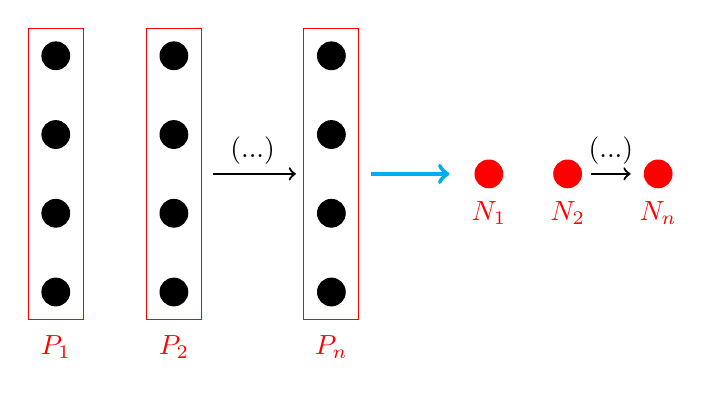
\begin{tikzpicture}[scale = 1.0]

\foreach \t in {0,1,...,3}
\filldraw[black] (0,{\t}) circle (5pt);
\foreach \t in {0,1,...,3}
\filldraw[black] (1.5,{\t}) circle (5pt);
\foreach \t in {0,1,...,3}
\filldraw[black] (3.5,{\t}) circle (5pt);
\draw[red] (-0.35,-0.35) rectangle (0.35,3.35);
\draw[red] (1.15,-0.35) rectangle (1.85,3.35);
\draw[red] (3.15,-0.35) rectangle (3.85,3.35);
\draw[thick,->] (2,1.5) -- (3.05,1.5);

\node at (2.5, 1.8) {(...)};
\node[red] at (0, -0.7) {$\text{P}_1$};
\node[red] at (1.5, -0.7) {$\text{P}_2$};
\node[red] at (3.5, -0.7) {$\text{P}_\text{n}$};

\draw[ultra thick,->, cyan] (4,1.5) -- (5,1.5);
\filldraw[red] (5.5,1.5) circle (5pt);
\filldraw[red] (6.5,1.5) circle (5pt);
\draw[thick,->] (6.8,1.5) -- (7.3,1.5);
\filldraw[red] (7.65,1.5) circle (5pt);

\node at (7.05, 1.8) {(...)};
\node[red] at (5.5, 1) {$\text{N}_1$};
\node[red] at (6.5, 1) {$\text{N}_2$};
\node[red] at (7.65, 1) {$\text{N}_\text{n}$};


\end{tikzpicture}
\caption{Plane assignment scheme.}
    \label{fig:ansys_python_mapping scheme_nodes}
\end{figure}